%! Date = 27/12/2024

% Preamble
\documentclass[11pt]{article}

% Packages
\usepackage{amsmath}
\usepackage{graphicx}
\usepackage{csvsimple}

%\newcommand{\projectroot}{.} % プロジェクトのルートディレクトリ
%\newcommand{\figurefilepath}{C:\Users\monyo\OneDrive - The University of Sydney (Staff)\PCS Library\figure\example_plot.pdf}

\usepackage[nonumberlist,nogroupskip]{glossaries}

\newglossaryentry{7730}
{
name={ISO~7730:2005},
description={ISO~7730:2005 is a thermal comfort standard developed by ISO}
}

\newglossaryentry{55}
{
name={ASHRAE~55--2020},
description={ASHRAE~55--2020 is a thermal comfort standard developed by ANSI and ASHRAE}
}

\makenoidxglossaries


% Document
\begin{document}
\title{Project Report 1: Research Questions for Environmental and Control Testing in PCS Evaluation}
\author{Akihisa Nomoto}
\date{\today}
\maketitle

%
\section*{Nomenclature}
\renewcommand{\baselinestretch}{0.75}\normalsize
\renewcommand{\aclabelfont}[1]{\textsc{\acsfont{#1}}}
\begin{acronym}[longest]

    \acro{t-eq}[$t_{eq}$]{equivalent temperature\acroextra{, $^{\circ}$C}}
    \acro{t-db}[$t_{db}$]{dry-bulb air temperature\acroextra{, $^{\circ}$C}}
    \acro{t-wb}[$t_{wb}$]{wet-bulb air temperature\acroextra{, $^{\circ}$C}}
    \acro{ti}[$t_{i}$]{indoor air temperature\acroextra{, $^{\circ}$C}}
    \acro{tout}[$t_{out}$]{outdoor air temperature\acroextra{, $^{\circ}$C}}
    \acro{t-op}[$t_{o}$]{operative air temperature\acroextra{, $^{\circ}$C}}
    \acro{t-cl}[$t_{cl}$]{clothing temperature\acroextra{, $^{\circ}$C}}
    \acro{tg}[$t_{g}$]{globe temperature\acroextra{, $^{\circ}$C}}
    \acro{rh}[$RH$]{relative humidity\acroextra{, \%}}
    \acro{v}[$V$]{average air velocity\acroextra{, m/s}}
    \acro{v-eq}[$t_{eq}$]{equivalent air velocity\acroextra{, m/s}}
    \acro{t-r}[$\overline{t_{r}}$]{mean radiant temperature\acroextra{, $^{\circ}$C}}
    \acro{clo}[$I_{cl}$]{total clothing insulation\acroextra{, clo}}
    \acro{i-cl}[$i_{cl}$]{permeation efficiency of water vapor through the clothing layer}
    \acro{met}[$M$]{rate of metabolic heat production\acroextra{, W/m\textsuperscript{2}}}
    \acro{work}[$W$]{rate of mechanical work accomplished\acroextra{, W/m\textsuperscript{2}}}
    \acro{t-sk}[$t_{sk}$]{skin mean temperature\acroextra{, $^{\circ}$C}}
    \acro{t-sk-n}[$t_{sk,n}$]{neutral skin mean temperature\acroextra{, $^{\circ}$C}}
    \acro{t-cr}[$t_{cr}$]{core mean temperature\acroextra{, $^{\circ}$C}}
    \acro{t-re}[$t_{re}$]{rectal temperature\acroextra{, $^{\circ}$C}}
    \acro{t-cr-n}[$t_{cr,n}$]{neutral core mean temperature\acroextra{, $^{\circ}$C}}
    \acro{r-cl}[$R_{cl}$]{thermal resistance of clothing\acroextra{, m\textsuperscript{2}K/W}}
    \acro{r-e-cl}[$R_{e,cl}$]{evaporative heat transfer resistance of clothing layer\acroextra{, m\textsuperscript{2}kPa/W}}
    \acro{f-cl}[$f_{cl}$]{clothing area factor $A_{cl}/A_{body}$\acroextra{, m\textsuperscript{2}K/W}}
    \acro{h}[$h$]{sum of convective $h_{c}$ and radiative $h_{r}$ heat transfer coefficients\acroextra{, W/(m\textsuperscript{2}K)}}
    \acro{h-r}[$h_{r}$]{linear radiative heat transfer coefficient\acroextra{, W/(m\textsuperscript{2}K)}}
    \acro{h-c}[$h_{c}$]{convective heat transfer coefficient\acroextra{, W/(m\textsuperscript{2}K)}}
    \acro{h-e}[$h_{e}$]{evaporative heat transfer coefficient\acroextra{, W/(m\textsuperscript{2}kPa)}}
    \acro{a}[$\alpha$]{fraction of the total body mass considered to be thermally in the skin compartment}

    \acro{cl-a}[$A_{cl}$]{clothing surface area\acroextra{, m\textsuperscript{2}}}

    \acro{e}[$\varepsilon$]{average emissivity of clothing or body surface}
    \acro{sigma}[$\sigma$]{Stefan-Boltzmann constant\acroextra{, 5.67 x 10\textsuperscript{-8} W/(m\textsuperscript{2}K\textsuperscript{2})}}

    \acro{a-r}[$A_{r}$]{effective  radiation  area  of  the  body\acroextra{, m\textsuperscript{2}}}
    \acro{body-a}[$A_{body}$]{body surface area\acroextra{, m\textsuperscript{2}}}
    \acro{body-w}[$mass$]{body mass\acroextra{, kg}}
    \acro{body-h}[$height$]{body height\acroextra{, m}}

    \acro{pmv}[PMV]{Predicted Mean Vote}
    \acro{ppd}[PPD]{Predicted Percentage of Dissatisfied\acroextra{, \%}}
    \acro{set}[SET]{Standard Effective Temperature\acroextra{, $^{\circ}$C}}
    \acro{ce}[CE]{Cooling Effect\acroextra{, $^{\circ}$C}}
    \acro{phs}[PHS]{Predicted Heat Strain}

    \acro{BMS}[BMS]{Building Management System}
    \acro{HVAC}[HVAC]{Heating, Ventilation, and Air Conditioning}
    \acro{VAV}[VAV]{Variable Air Volume}
    \acro{AHU}[AHU]{Air Handling Unit}

    \acro{ema}[EMA]{Ecological Momentary Assessment}
    \acro{sdk}[SDK]{Software Development Kit}
    \acro{api}[API]{Application Programming Interface}

    \acro{s-cr}[$S_{cr}$]{rate of heat storage in the core compartment\acroextra{, W/m\textsuperscript{2}}}
    \acro{s-sk}[$S_{sk}$]{rate of heat storage in the skin compartment\acroextra{, W/m\textsuperscript{2}}}
    \acro{s}[$S$]{rate of heat storage in the human body\acroextra{, W/m\textsuperscript{2}}}
    \acro{e-res}[$E_{res}$]{rate of evaporative heat loss from respiration\acroextra{, W/m\textsuperscript{2}}}
    \acro{e-dif}[$E_{dif}$]{rate of evaporative heat loss from moisture diffused through the skin\acroextra{, W/m\textsuperscript{2}}}
    \acro{e-rsw}[$E_{rsw}$]{rate of evaporative heat loss from sweat evaporation\acroextra{, W/m\textsuperscript{2}}}
    \acro{e-sk}[$E_{sk}$]{total rate of evaporative heat loss from skin\acroextra{, W/m\textsuperscript{2}}}
    \acro{e-max}[$E_{max}$]{maximum rate of evaporative heat loss from skin\acroextra{, W/m\textsuperscript{2}}}
    \acro{c-res}[$C_{res}$]{rate of convective heat loss from respiration\acroextra{, W/m\textsuperscript{2}}}
    \acro{c-r}[$C + R$]{sensible heat loss from skin\acroextra{, W/m\textsuperscript{2}}}
    \acro{q-res}[$q_{res}$]{total rate of heat loss through respiration\acroextra{, W/m\textsuperscript{2}}}
    \acro{q-sk}[$q_{sk}$]{total rate of heat loss from skin\acroextra{, W/m\textsuperscript{2}}}
    \acro{w}[$w$]{skin wettedness}
    \acro{w-max}[$w_{max}$]{skin wettedness practical upper limit}
    \acro{m-sweat}[$m_{rsw}$]{rate at which regulatory sweat is generated\acroextra{, mL/h\textsuperscript{2}}}
    \acro{m-bl}[$m_{bl}$]{skin blood flow\acroextra{, L/(hm\textsuperscript{2})}}
    \acro{c-sw}[$c_{sw}$]{driving coefficient for regulatory sweating\acroextra{, g/(hKm\textsuperscript{2})}}

    \acro{p-sk}[$p_{sk,s}$]{water vapor pressure at skin\acroextra{, kPa}}
    \acro{p-a}[$p_{a}$]{water vapor pressure in ambient air\acroextra{, kPa}}

    \acro{wmo}[WMO]{World Meteorological Organization}
    \acro{who}[WHO]{World Health Organization}
    \acro{cdc}[CDC]{Centers for Disease Control and Prevention}
    \acro{noaa}[NOAA]{National Oceanic and Atmospheric Administration}
    \acro{epa}[EPA]{United States Environmental Protection Agency}
    \acro{iea}[IEA]{International Energy Agency}
    \acro{un}[UN]{United Nations}

\end{acronym}
\renewcommand{\baselinestretch}{1}\normalsize


\section*{Overview}

In this project, we aim to develop a database for thermal environmental changes surrounding the human body when using a Personal Comfort System (PCS).
This database will help researcher understand the impact of PCS on thermal comfort and be a valuable resource for comfort simulations.

This report examines our research questions and proposes a standardized method and explores its limitations. This work will help resersher to jump in this project before developing the database.
Probably the next report will be a database focusing on the typical office PCS.


\section*{Key Research Questions}

\begin{enumerate}
    \item \textbf{Temperature Dependence of Testing Environments}
    : Is there a temperature dependence in the surrounding environment?
    \begin{itemize}
        \item Verify whether there is a difference in overall heat transfer coefficient between clothed and unclothed conditions.
        \item There is if air movement is provided because the convective heat transfer depends on the ambient temperature, but may be less when warming PCS is used.
    \end{itemize}

    \item \textbf{Clothing Dependence}
    : Airflow passes through fabric fibers, so it is desirable to measure conditions assuming actual clothing. However, this means that changing the clothing alters the results, which may limit generalizability.
    It might be good idea to test using different clothing ensambles that we could think of, and then show the variety of effects (e.g. 0.3-0.4 m/s).
    \begin{itemize}
        \item Investigate the difference in the impact of PCS when clothing differs at a given temperature.
        \item Might be good to have a standalized clothing ensambles for both summer and winter. UNIQLO's clothing might be good idea because it is around the world, which makes the dupulication easy.
    \end{itemize}

    \item \textbf{Manikin’s Control Method}
    : There are (1) surface temperature control, (2) heat flux control, and (3) comfort control methods. Temperature control with PI control is easier to interpret. Can the same results be obtained with comfort control?
    \begin{itemize}
        \item At a given temperature, examine the impact of PCS under surface temperature control and comfort control conditions.
    \end{itemize}

    \item \textbf{Output Results}
    : What should be organized as output results?
    \begin{itemize}
        \item Considering input conditions for modeling, it may be ideal to organize results based on changes in $\Delta X$. Maybe, using $\Delta t_{eq}$ would be the simplest approach?
    \end{itemize}

\end{enumerate}


\subsection{Figure}
\begin{figure}[h!]
    \centering
    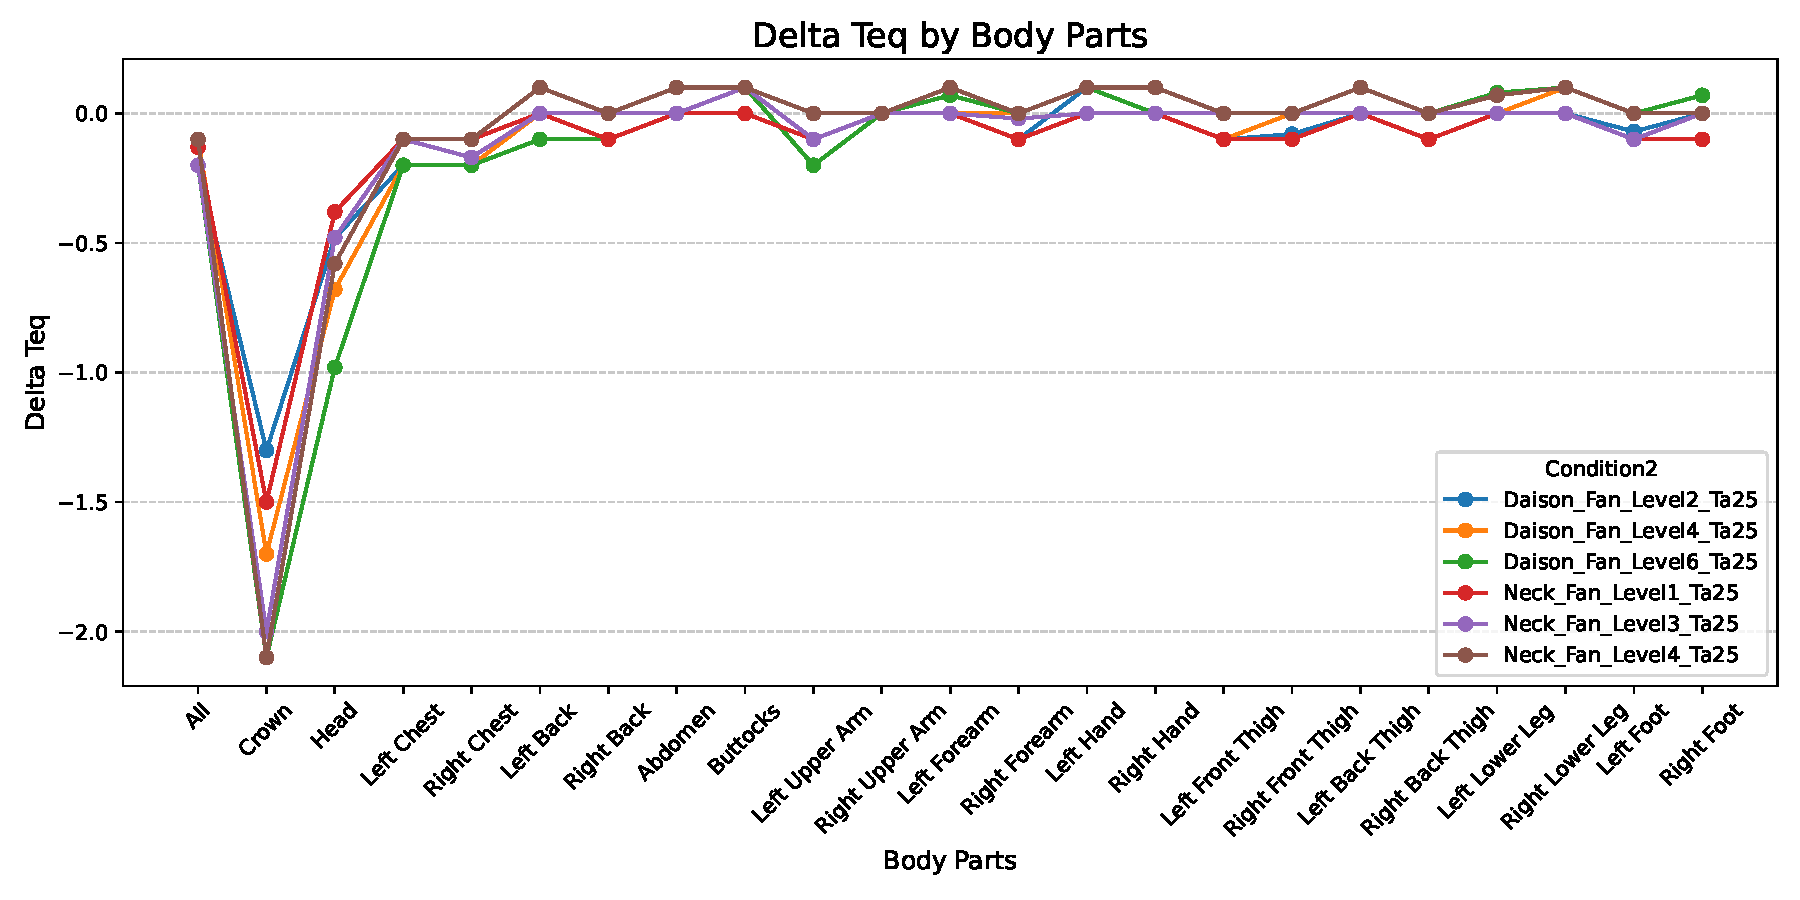
\includegraphics[width=0.8\textwidth]{C:/Users/monyo/OneDrive - The University of Sydney (Staff)/PCS Library/figure/example_plot.pdf}
    \caption{Example PDF Figure}
    \label{fig:example}
\end{figure}



\section*{Other variables}

\begin{enumerate}
    \item \textbf{Noise level}

\end{enumerate}
%\subsection{How to add acronyms/nomenclature}\label{subsec:how-to-add-acronyms}
%This is an example on how to add acronyms.
%You can reference the acronym using the command \verb!\ac{t-db}! this will result in the following \ac{t-db}.
%If you use the command \verb!\ac{t-db}! again, it will result in \ac{t-db}.
%You can check the list of acronyms in the \texttt{myacronyms.tex} file.
%
%\subsection{Glossary}\label{subsec:glossary}
%
%This is an example on how to add a glossary.
%You can reference the glossary using the command \verb!\gls{7730}! this will result in the following \gls{7730}.
%You can check the list of glossary terms in the \texttt{myglossary.tex} file.

\end{document}
